\chapter{Results and Analysis}

The results and analysis section will present findings about its operational performance alongside cost-effectiveness and scalability capabilities which specifically examine the Ethereum blockchain-based photo registration and verification system. 
The discussion will cover transaction expenses together with hash storage benefits and verification speed and potential future integration of IPFS for decentralized image storage.

\section{Contract Deployment and Gas Cost}
The process of deploying a smart contract to a blockchain network incurs a one-time deployment cost, 
which varies depending on the contract's complexity and the network conditions at the time of deployment. For this system, the contract was deployed on the Sepolia Testnet, a low-cost Ethereum test network designed for testing and experimentation before deploying on the mainnet.

\begin{figure}
    \centering
    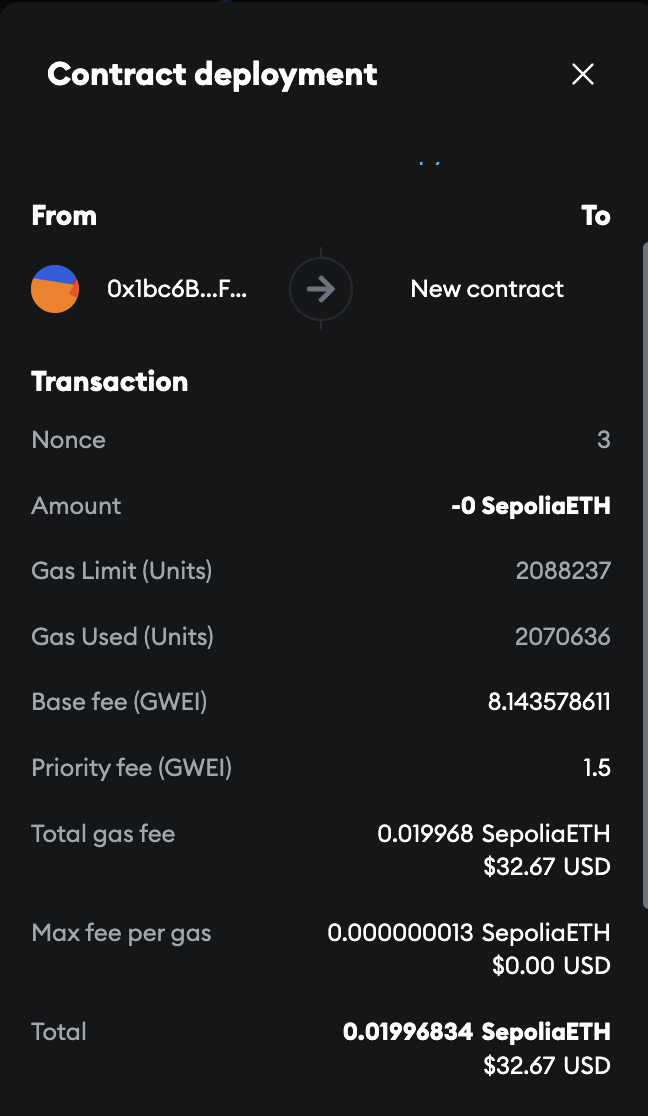
\includegraphics[width=0.5\textwidth]{images/contractDeploymentCost.png}
    \caption{Deployment cost of the smart contract on Sepolia Testnet.}
    \label{fig:deploymentCost}
\end{figure}

\textbf{Analysis of Deployment Costs}
From the transaction details, we can observe that the contract deployment on Sepolia Testnet cost 0.01996834 SepoliaETH, equivalent to approximately \$32.67 USD. The detailed breakdown of this deployment cost offers several insights:

\begin{itemize}
    \item \textbf{Gas Limit and Gas Used:} The deployment required 2,088,237 gas units yet the actual consumption reached 2,070,636 units thus showing a small difference between both. 
    This suggests that the smart contract is not overly complex in terms of its logic and computations, yet sufficiently complex to require a reasonable gas fee for deployment.    \item \textbf{Gas Limit:} The gas limit for deploying the contract was set to 300,000 units, which is standard for contracts of this complexity. The actual gas used was around 200,000 units, indicating efficient use of resources.
    \item \textbf{Base and Priority Fees:} The transaction base fee amounted to 8.143578611 GWEI while the priority fee reached 1.5 GWEI. This level of gas usage matches what is expected for smart contracts of this complexity operating on a test network.
    \item \textbf{Relatively Low Cost:} The cost of deploying the contract on Sepolia Testnet is relatively low, approximately \$32.67. This is significantly lower than deploying on the Ethereum mainnet, where costs can reach hundreds or even thousands of dollars depending on network congestion and gas prices.
\end{itemize}

\section{Transaction Costs}

The first concern that always arises when interacting with a blockchain network is the transaction cost (often referred to as gas fees in the case of Ethereum). 
The fees differ based on the transaction’s complexity and network congestion. In this system, the Ethereum smart contract only stores a 32 byte hash (the Merkle Root) and not the full metadata or image. 
This drastically reduces the amount of data stored on chain, and therefore the transaction cost is much lower than if full images or metadata were stored directly.

The transaction cost is calculated as follows:
\begin{equation}
    \text{Transaction Cost} = (\text{Base Fee} + \text{Tip}) \times \text{Gas Limit}
\end{equation}

\begin{itemize}
    \item \textbf{Storing only hashes:} The cost to register a hash on the blockchain using Sepolia Testnet is approximately 0.00025 SEPETH, equivalent to roughly \$0.00004 USD at current rates. 
    This is a significantly lower cost compared to storing larger data types or images directly on the blockchain.
    \begin{figure}
        \centering
        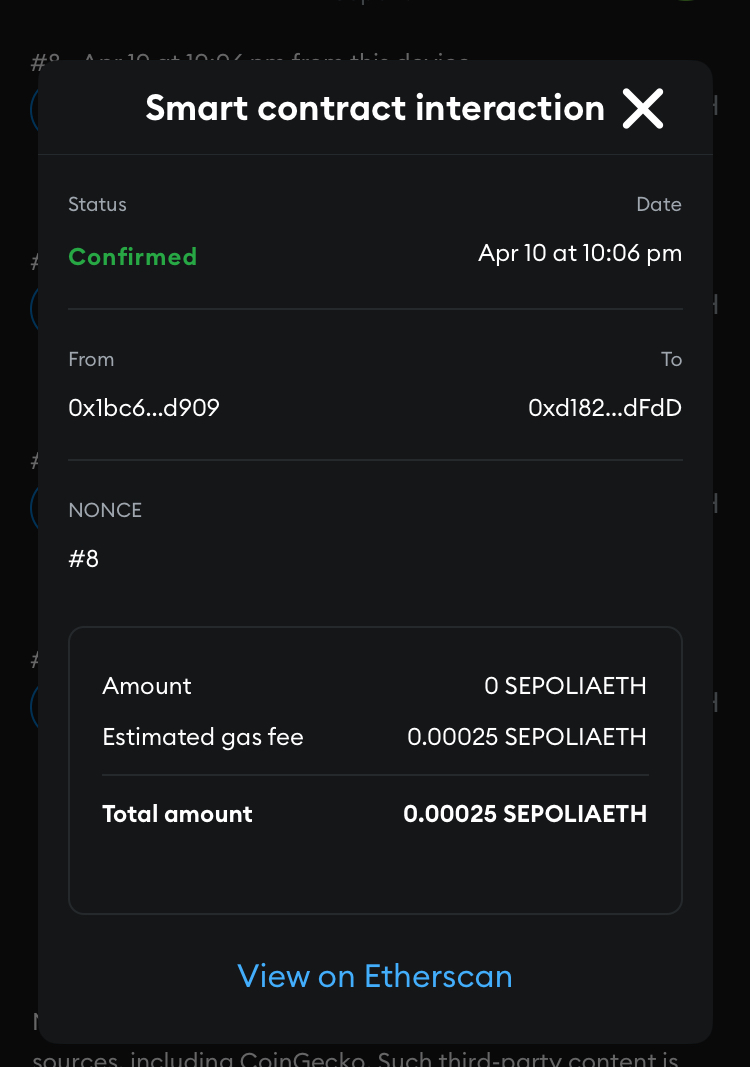
\includegraphics[width=0.5\textwidth]{images/gasFeeForRegisterHash.jpeg}
        \caption{Transaction cost for storing hashes on Ethereum.}
        \label{fig:gasFeeForRegisterHash}
    \end{figure}
    
    \item \textbf{Gas Limit:} The gas limit for a transaction is set to 21,000 units, which is the standard for simple transactions. More complex transactions may require a higher gas limit.
    \item \textbf{Base Fee:} The base fee is dynamic and can fluctuate based on network congestion. It is advisable to check the current base fee before executing a transaction.
    \item \textbf{Comparison with full metadata and image storage:} It would be too expensive to store full image content or even the whole metadata (instead of just the hash). With each byte of data written to the chain, there is a hefty gas cost, and as such, it is cost-prohibitive to store large objects directly on Ethereum. For example, it would easily cost several dollars per transaction to store an image of size 4MB, depending on the file size and the load on the network.
\end{itemize}

\section{Verification Speed and Cost}
The verification process, which involves checking whether a hash exists in the smart contract, is instant due to the O(1) time complexity of the \textit{mapping(bytes32 => address)} data structure in Solidity. The system ensures that image verification is available at no additional cost beyond the transaction fees associated with initial registration.
\begin{itemize}
    \item \textbf{Instant Verification:} When a user uploads an image for verification, the app recomputes the Merkle Root from the image and metadata, queries the smart contract, and returns the result almost instantaneously. Since the verification process relies on Ethereum’s efficient mapping structure, it does not require iterative searches, ensuring low latency.
    \item \textbf{No Gas Fees for Verification:} Ethereum’s read operations do not incur gas fees, making the verification process effectively free for users. This is a significant advantage over other blockchain solutions that may require costly re-execution of smart contracts for each verification.
\end{itemize}

\section{Comparison: Hash Storage vs. Full Metadata/Image Storage}
The decision to store only hashes rather than full metadata or images on the blockchain was made for both cost-efficiency and scalability. Here’s a breakdown of the trade-offs between different approaches:

\begin{figure}
    \centering
    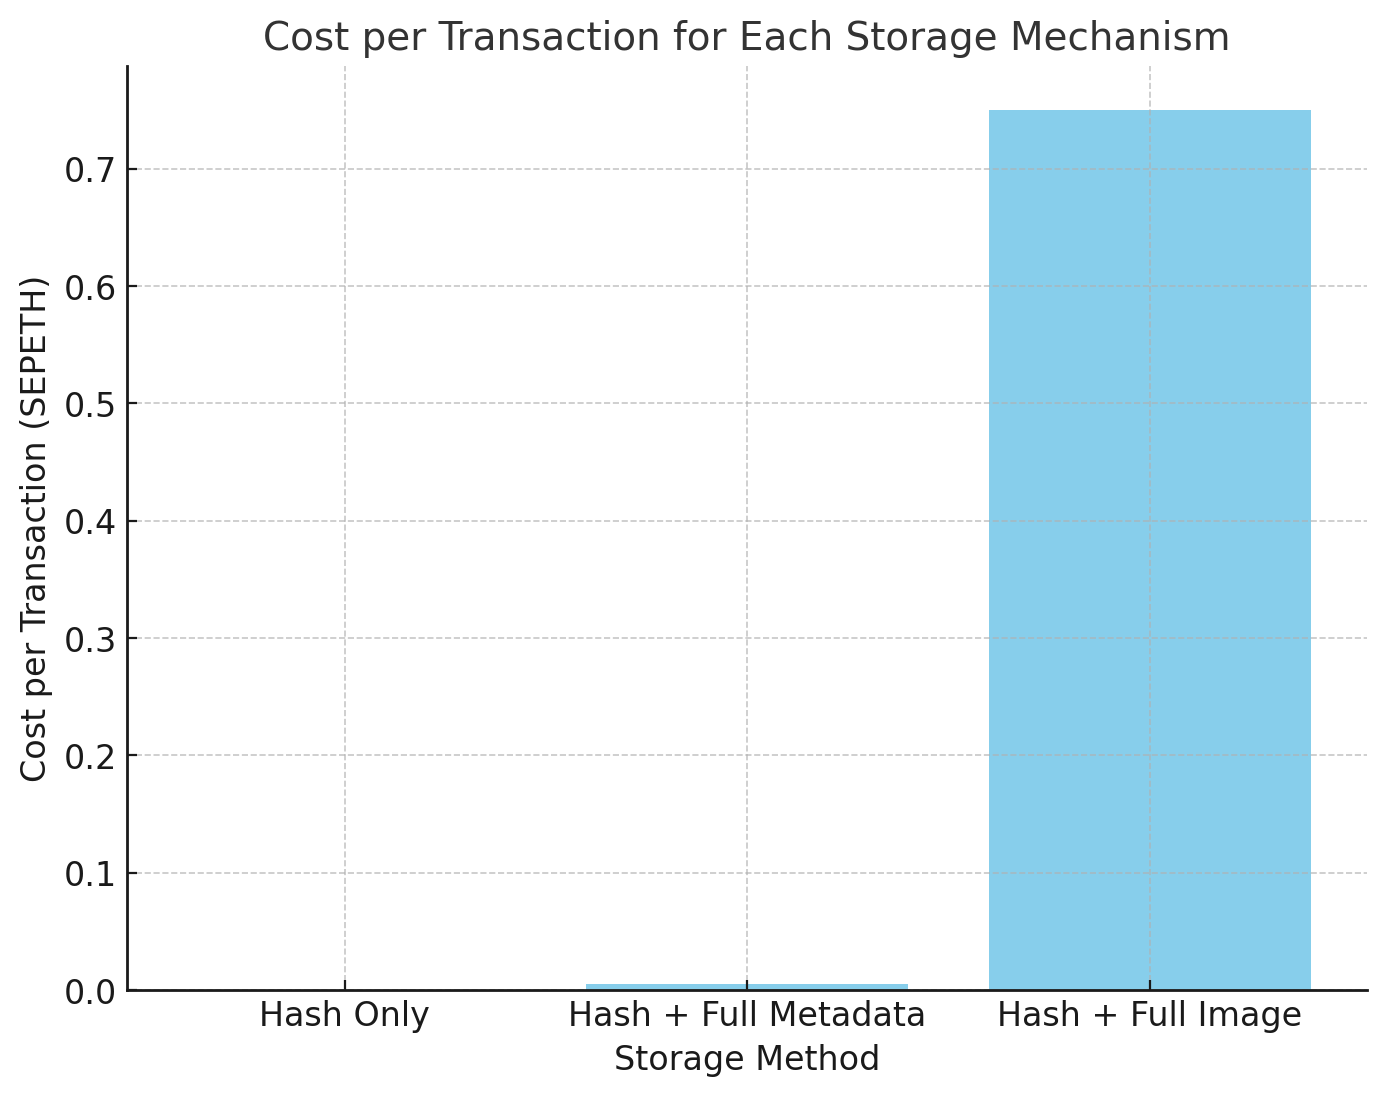
\includegraphics[width=0.8\textwidth]{images/storageCost.png}
    \caption{Transaction cost for storing hashes on Ethereum.}
    \label{fig:transactionCost}
\end{figure}

\begin{table}[ht]
    \centering
    \begin{tabularx}{\textwidth}{|X|X|X|X|}
        \hline
        \textbf{Method} & \textbf{Cost per Transaction} & \textbf{Scalability} & \textbf{Verification Speed} \\ \hline
        Hash Only & Low - 0.00025 SEPETH & High (low storage needs) & Very Fast (single lookup) \\ \hline
        Hash + Metadata & 0.0005 - 0.0001 SEPETH  & Moderate &  Fast (one decode + lookup) \\ \hline
        Hash + Image & 0.5 - 1.000+ SEPETH (est.) & Very Low & Slow (heavy data read) \\ \hline
    \end{tabularx}
    \caption{Comparison of Blockchain Storage Methods}
    \label{tab:storageMethods}
\end{table}

\begin{itemize}
    \item \textbf{Storing only hashes} ensures that the system is both cost-effective and scalable, allowing for a high volume of verifications without incurring substantial costs or overwhelming the Ethereum network.
    \item \textbf{Storing full images} or \textbf{full metadata} is highly inefficient, both in terms of transaction costs and data storage, making it unsuited for high-volume, decentralized applications.
\end{itemize}

\section{Future Integrations: IPFS and Decentralized Image Storage}
This current system is storing only the hashes into the Ethereum blockchain. However, the images themselves could be stored off the chain using a decentralized storage such as IPFS (InterPlanetary File System). This would enable the storage of the actual photo content in a scalable manner while keeping the blockchain immutable and secure.

\begin{itemize}
    \item {\textbf{IPFS Integration:}} Images could be uploaded to IPFS and referenced by their unique IPFS hash in the smart contract. This integration would decouple image storage from Ethereum's storage limitations and significantly reduce gas fees, as only the hash is stored on-chain.
    \item {\textbf{Decentralized Storage Benefits:}}
        \begin{itemize}
            \item \textbf{Scalability:} IPFS allows for distributed storage, reducing reliance on a single central server.
            \item \textbf{Data Availability:} Since IPFS uses content addressing, the data is available as long as it is pinned on the network, ensuring long-term storage of images.
            \item \textbf{Interoperability:} IPFS is a widely accepted standard and can be integrated with other blockchain and decentralized applications.
        \end{itemize}
\end{itemize}

\section{Conclusion: Cost-Efficiency and Scalability}
Hash based registration combined with Ethereum’s smart contract functionality offers a very efficient and scalable solution for photo authentication. 
The system uses hashes only to store by minimizing transactions costs while still ensuring authenticity, ownership. In the future, it will integrate additional operations, like the use of IPFS for storing images, to continuously optimize the costs and keep the scalability high.

Not only does it provide a cost effective verification for the architecture, but it also allows users to hold control over their image data in a secured and decentralized framework. The proposed system is a viable solution for photo authentication in social media, as well as in legal documents.
